% 
% %\documentclass[paper=a4,fontsize=12pt,open=right,noabbrev]{report}
% \documentclass[12pt]{report}
% \usepackage[utf8]{inputenc}
% \usepackage{amsmath}
% \usepackage{amssymb}
% \usepackage{graphicx}
% \usepackage{cite}
% \usepackage{physics} 
% \usepackage{mathrsfs}
% \newcommand*\diff{\mathop{}\!\mathrm{d}}
% \usepackage{geometry}
% \usepackage{layouts}
% \usepackage{newfloat}
% \usepackage{float}
% \usepackage{listings}
% \usepackage{bm}
% \usepackage{csquotes}
% 
% \setlength{\parindent}{0em}
% \setlength{\parskip}{1em}
% 
% \lstset{language=Python,basicstyle={\ttfamily }}
% 
% %% Technical point floatstyle
% \floatstyle{ruled}
% \newfloat{Technical Point}{htbp}{lop}[chapter]
% 
% 
%  

%\begin{document}

\chapter{Jaynes Maximum Caliber}
\label{ch:Jaynes}
Edwin Thompson Jaynes discussed the question of the possibility of macroscopic 
prediction from microscopic information of a system~\cite{jaynes1985macroscopic}. He based 
his work on the earlier theory of  Boltzmann's statistical 
mechanics~\cite{boltzmann1896vorlesungen}. Boltzmann stated that the entropy 
is the crucial key to connect microscopic and macroscopic phenomena --- and that the 
lack of understanding a macroscopic phenomena might be caused 
by ignoring the effect of the entropy. Boltzmann connected the two worlds by 
the simple identity $S = k_{\textrm{B}} \ln{W}$, where the 
left-hand side  is the macroscopic property entropy, known from equilibrium thermodynamics, and the right-hand side counts the number of microscopic 
configurations. The argumentation transformed time-dependent trajectories to a 
collection of microstates and thus ergodicity was demanded. 

Gibbs introduced the idea of probabilities of a microstate 
$i$ in an entropic 
system in the form of $S = -k_{\mathrm{B}} \sum_i p_i \ln p_i$. He changed the point of view by the introduction of ensembles with certain thermodynamic characteristics, like constant temperature or pressure. 
The ensembles allow us to observe a number of identical non-interacting systems with the same macroscopic parameters instead the time-evolution of a single system. The axiom of \textit{equal a priori probabilities} becomes necessary. It states that all known states have the same probability without further knowledge of the system to connect the independent system, i.e. $p_i = \frac{1}{W}$. The Gibbs formulation of the entropy reduces to Boltzmann's formula 
\begin{equation}
\begin{aligned}
 S &= -k_{\mathrm{B}} \sum^W_i p_i \ln p_i \\
 & = -k_{\mathrm{B}} \sum^W_i \frac{1}{W} \ln \frac{1}{W} \\
 & =k_{\mathrm{B}} \ln W,
\end{aligned} 
\end{equation}
meaning that Boltzmann's equation holds for no additional thermodynamic information. In the Gibbs formulation, the entropy decreases if information are given,   resulting in probabilities of microstates that differ from one another. He shows how to introduce statistical ensembles (see section~\ref{sec:EnsembleAv}) in equilibrium by maximising the entropy with respect to certain constraints~\cite{gibbs1902elementary}. He claims that a statistical system is observed in a state where it has the most microscopic realisations available while satisfying macroscopic constraints. Other states may agree with these constraints but are entropically suppressed and are thus negligible. 
 
\begin{Technical Point}[t] 
\begin{minipage}{0.03\textwidth}
\hfill\vspace{0.1cm}
\end{minipage}%
\begin{minipage}{0.4\textwidth}
 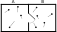
\includegraphics{../images/maxwell.pdf}
\end{minipage}
\hfill
\begin{minipage}{0.55\textwidth}
  Maxwell proposed a gedankenexperiment that seemingly opposes the second law of thermodynamics. He assumed two boxes A and B that are filled with particles and only connected by a door that can be opened and closed.  Assuming the existence of a all-knowing conscious --- the demon --- it could open the door whenever a fast particle passes from  box A to B and close
  it otherwise. In the other direction,  it could \vspace*{0.055cm} \end{minipage}  open the door whenever a slow particle wants to pass from box B to A and close it otherwise.
  The door operates frictionless. The box A would cool down and B would heat up --- opposing the second law of thermodynamics which demands that two objects in contact evolve to an equilibrium with both objects at the same temperature~\cite{leff2014maxwell}. \\
  
  It is believed that the laws of thermodynamics are not violated, but it follows that a source of the missing entropy production, to fulfil $\delta S \ge 0$, is missing. The source is found in the demon itself, which interacts with the system by measurement and by storing data. The measurement can be ruled out because it was shown to be possible by a reversible process~\cite{landauer1961irreversibility}. A solution identified by Bennett states that the demon eventually runs out of data storage and has to delete gathered information~\cite{bennett1987demons}. Laundauer showed that deleting one bit increases the entropy by $S_{\text{bit}} = k_{\mathrm{B}}\ln 2$~\cite{bennett2003notes}. The gedankenexperiment of Maxwell's Demon provides us with a way to think of the connection of information and physical entropy.  
  \caption{Maxwell's Demon}\label{tec:Maxwell}
\end{Technical Point}
 
Shannon introduced the information-theoretic entropy for a probability distribution given by $S = \sum_i p_i \log_2 p_i$, only differing from the Gibbs entropy by the factor of $k_B \ln 2$~\cite{shannon1948mathematical}. 
The Gibbs entropy can be seen as the amount of Shannon entropy required to define the microscopic state of a system. The reverse consequence --- that the possession of microscopic information must have thermodynamic consequences --- was formulated in the form of the famous Maxwell Demon~\cite{bennett1982thermodynamics} (see technical point~\ref{tec:Maxwell} ). Jaynes accepted the similarity of information and thermodynamic entropy without proof and proposed to generalise the Gibbs algorithm from thermodynamic systems to all probabilistic systems. In a first step, he formulated this idea for equilibrium systems \cite{jaynes1957information}, later he extended it to time-depending off-equilibrium  systems~\cite{jaynes1985macroscopic}. His idea is to move from a physical deductive theory for thermodynamics to an inferent theory: A deductive theory predicts what will happen, whereas the inference theory proposes the most likely probability distribution based on given data and information. 
He also argues from a practical way that most real systems are 
too complex for a deductive proof with definite predictions. Most important 
is the correct identification of macroscopic parameters that reduce the information entropy to a significant distribution of microstates. From the remaining probability distributions that fulfill the constraints, the one with the highest entropy (or least information) is chosen to be as non-committal as possible with regard to unknown information. Insignificant information 
on the other hand will barely change the outcome compared to the prior information.
This information-theoretic argumentation allows to drop the assumption of equal a priori probabilities and ergodicity. The first assumption is now a product of the theory in case when no information are available: The entropy function $-k_{\mathrm{B}} \sum^W_i p_i \ln p_i$ has a global maximum for equal probabilities $p_1 = p_2 =\dots=p_W$.  The second assumption of ergodicity was initially introduced to describe equilibrium systems by their microstates instead of time-dependent trajectories.  The shift from a physical theory to an information theory makes this assumption obsolete. We may apply the theory to any kind of probabilistic systems including fields in physics, biology, economics and more. 

Later, Shore and Johnson changed the point of view on the maximum entropy assumption once more: They showed that the entropy function by Shannon is the only function that fulfils logical requirements of inference, 
as it will be shown in the following section~\ref{sec:inference}. It proves that the argument of maximising the uncertainty of Jaynes is not needed anymore. The maximum uncertainty is a necessary criterion for a consistent inference method. 

Depending on the situation of the inference task, one might 
use any of the given interpretation by Gibbs, Jaynes or by Shore and Johnson. 
The Gibbsian point of view is motivated by physics and provides a good 
basis for the interpretation of equilibrium statistical physics. Jayne's method 
allows an interpretation of all fields beyond equilibrium physics, whereas Shore's and Johnson's addition to the theory base it on a solid logical ground but is less applicable for a physical interpretation. This thesis uses the name \textit{Maximum Caliber} for historical reasons, although other mathematicians and physicists than Jaynes contributed to understanding the method.  



\section{Requirement for uncertainty measures and inference methods}
\label{sec:inference}
% uncertainty measure - NOT fulfiled by Bayes? % shift to KL-diveregence
% SJ : properties of inference method - Is this fulfilled by Bayes?
There are numerous functions that may be considered as a measure for uncertainty.
This thesis focuses on the relative entropy as defined by Kullback and Leibler 
$ \int_X \dd{X} P(X) \ln \frac{P(X)}{Q(X)}$, where $Q(X)$ represents the assumed distribution called \textit{prior} in Bayesian statistics. $P(X)$ is the probability distribution assigned based on the data and constraints, called \textit{posterior}~\cite{jaynes2003probability}. It fulfils the axioms an uncertainty measure should meet as formulated by Hobson~\cite{hobson1973comparison} as an extension to Shannon's axioms~\cite{shannon1948mathematical}. 
The extension was necessary to include known data that 
was not considered by the entropy definition of Jaynes. 
The uncertainty measure is denoted by $S(P(X)|Q(X))$, where
the probability of outcome $X= (x_1, x_2,...,x_N)$ is $P(X)$, assuming prior $Q(X)$. An uncertainty measure should fulfil the following axioms:
\begin{itemize}
 \item 1. $S(P(X)|Q(X))$ is continuous in $P(X)$ and $Q(X)$.
 \item 2. $S(P(X)|Q(X))$ does not depend on how the outcome $x_1,x_2, ... , x_N$ 
 are labeled.
 \item 3. $S(P(X)|Q(X)) = 0$ if $P(X) = Q(X)$ 
 \item 4. When $Q(X) = (n_0^{-1}, n_0^{-1} , ... , n_0^{-1})$ and 
 $P(X) = (n^{-1}, n^{-1} , ... , n^{-1},0,...,0)$ $(n \leq n_0)$ then 
 $S(P(X)|Q(X))$ is an increasing function of integer $n_0$ and decreasing function of $n$.  
\item 5. If $Y$ denotes additional states and $P(X,Y)$ and $Q(X,Y)$ denote the 
joint probabilities, then the uncertainty of the composite system should be expressed as
\begin{equation}
   S(P(X,Y)|Q(X,Y)) = S(P(X)|Q(X)) + \sum_i P(x_i) S(P(Y | x_i) | Q(Y | x_i)) % is this correct..? 
\end{equation}
\end{itemize}
The first three axioms are reasonable, only defining a continuous function with a minimum whenever $P(X)$ equals $Q(X)$, meaning no new information are given  
and the ordering of learning new variables does not matter.
The forth axiom states that uncertainty decreases if states can be deleted and increases if states 
are introduced. 
% think about the last axiom
The last axiom defines the extension of correlated systems, where 
the uncertainty should grow with additional states $y_i$ consistent with the conditional probability $p(y_1,..., y_M | x_i)$.
The Kullback-Leibler entropy in the form of
\begin{equation}
 S(P(X)|Q(X)) = \int \dd{X}  P(X) \ln \frac{P(X)}{Q(X)} 
\end{equation}
is the unique functional form for an uncertainty measure fulfilling above axioms. The negative Kullback-Leibler divergence (or relative entropy) reduces to the Shannon entropy 
if the prior is equi-distributed~\cite{shannon1948mathematical}.
Hobson shows that the Kullback-Leibler divergence has a unique minimum for $Q(X) = P(X)$ and it is convex in the sense of probability mass functions. 
To apply Jaynes theory, we will use a prior to include data on the system and constraints in the form of Lagrangian multipliers to infer physical information. The result of this inferring process should follow some axioms too, as formulated and proven for the Kullback-Leibler divergence by Shore and Johnson~\cite{shore1980axiomatic}:
\begin{itemize}
 \item Uniqueness: The result should be unique.
 \item Invariance: The result is independent of the choice of the coordinate system.
 \item System Independence: Independent information about independent systems can be inferred separately in terms of different densities or together in terms of joint densities.
 \item Subset Independence: Independent subsets of system states can be treated in terms of a separate conditional density or in terms of the full density. 
\end{itemize}
All axioms together lead to the Kullback-Leibler divergence as the unique consistent candidate for inferring information on a set of data. We showed before that it is also a function for uncertainty measurement, supporting Jaynes intuitive interpretation of choosing the system of highest uncertainty under defined constraints.
 
The assumptions made above do not require equilibrium of any kind. We will continue 
to show how the Maximum Caliber with an equilibrium assumption is used to derive ensembles in statistical mechanics and continue by generalizing to off-equilibrium steady states. 

\section{Reweighting in Equilibrium}
 \label{sec:rewEqu}

The following derivation shows how Jaynes principle is used to recover data reweighting (see section~\ref{sec:EnsembleAv}), a method that was first described by Swendsen and Ferrenberg and is frequently used for simulation~\cite{ferrenberg1988new}. 
According to Gibbs statistical ensembles, a canonical ensemble (or $NVT$ ensemble) is defined by a closed system of constant volume, that does not allow particle exchange with its surrounding and is connected to an infinitely large reservoir with constant temperature and can exchange energy with it. Applying Jaynes theory, we infer the macroscopic average energy of the system. 
It is assumed that microscopic data is available from previous measurements in form of $q(x)$, where $x$ is a microstate with Energy $E(x)$. Considering the information, the Caliber is denoted by
\begin{equation}
\begin{aligned}
\mathcal{C_{\text{equ}}} = -\int \diff x \; p(x) \ln \left ( \frac{p(x)}{q(x)} \right )  - \zeta \left ( \int \diff x \; p(x) - 1 \right ) \\
- \beta \left( \int \diff x \; p(x) E(x) - \langle E \rangle \right),
\end{aligned}
\label{eq:Caliber1}
\end{equation}
where $\zeta$ and $\beta$ denote Lagrangian multipliers and the probability distribution $p(x)$ is normalised to $1$.  Functional maximisation $\fdv{\mathcal{C_{\text{equ}}} }{p(x)} = 0$ yields 
\begin{equation}
 p(x) = q(x) \exp \left ( -1 - \zeta -\beta E(x) \right ).
\end{equation}
Enforcing normalisation to $1$ gives an expression for the corresponding Lagrangian multiplier $\zeta$. One finds an expression for the new probability distribution that depends on $\beta$
\begin{equation}
    p(x) =  \frac{q(x) \exp \left ( -\beta E(x) \right )}
    {\int \diff x q(x) \exp \left( -\beta E(x) \right ) }. 
\label{eq:RewEqu}
\end{equation}
This is the reweighting formula for reference data $q(x)$ to $p(x)$ based on a change in the average energy. From equilibrium statistical mechanics (see section~\ref{sec:EnsembleAv}) we know that the Lagrangian multiplier $\beta$ can be identified with the inverse temperature  $ \frac{1}{k_{\textrm{B}}T}$ that controls the average energy in a canonical ensemble. The reweighting procedure connects the probability distributions at different temperatures. 
\begin{Technical Point}[t]
\begin{minipage}{0.03\textwidth}
\hfill\vspace{0.1cm}
\end{minipage}%
\begin{minipage}{0.3\textwidth}
    \includegraphics{../images/ISAW.pdf}
\end{minipage}
\hfill
\begin{minipage}{0.65\textwidth}
The self-avoiding walk (SAW) was introduced by Paul Flory to model chain-like polymers~\cite{flory1953principles}. The polymer is mapped on a grid where each site represents one monomer. An already occupied site cannot be \vspace*{0.055cm} \end{minipage} occupied  by another monomer to model the self-excluding interaction. An interaction between close-by monomers is introduced by an attractive potential between monomers on neighbouring sites. For $n_b$ bonds of strength $J$ one finds the energy


\begin{equation}
 E = -J n_b .
\end{equation}
The model can be constructed on different grids, however their effects on the system vanish in the thermodynamic limit~\cite{de1979scaling}. The SAW was studied in various dimension,  with different interaction range or close to surfaces and has become one of the most-studied models in polymer physics~\cite{vanderzande1998lattice}. 
  \caption{Interacting Self-Avoiding Walk}\label{tec:ISAW}
\end{Technical Point}
It can be understood by assuming that the reference data was sampled from a canonical ensemble at temperature $T'$, i.e. $q(x) = \exp \left ( \frac{-E(x)}{k_{\mathrm{B}} T'} \right )$. Plugging this into equation~\ref{eq:RewEqu}  shows that 
\begin{equation}
     p(x) =  \frac{ \exp \left [ \left ( -\frac{1}{k_{\mathrm{B}} T} - \frac{1}{k_{\mathrm{B}} T'} \right )E(x) \right ]}
    {\int \dd{x} \exp \left [ \left ( -\frac{1}{k_{\mathrm{B}} T} - \frac{1}{k_{\mathrm{B}} T'} \right )E(x) \right ] }
\end{equation}
is the probability distribution at a a new temperature $T'' = \frac{1}{\frac{1}{T'}+\frac{1}{T}}$. We conclude that the chosen temperature $T$, or the Lagrangian multiplier $\beta$, in the reweighting procedure is the change in temperature from the reference data. Making use of the density of states $\Omega(E)$ the reweighting equation~\ref{eq:RewEqu} recovers the known relation 
\begin{equation}
     p(E) =  \frac{ \Omega(E) \exp \left [ \left ( -\frac{1}{k_{\mathrm{B}} T''} \right )E \right ]}
    {\int \dd{E} \Omega(E) \exp \left [ \left ( - \frac{1}{k_{\mathrm{B}} T''} \right )E \right ] }.
\end{equation}
Here we assume that the density of states is fully known. However, since we only have access to the reference data $q(x)$ the density of states is only estimated over a sampled region by
\begin{equation}
 \Omega(E) \approx \int \dd{x} \delta(E(x) - E) \exp \left ( \frac{E(x)}{k_{\mathrm{B}} T} \right ).
\end{equation}
This sampling issue is illustrated in figure~\ref{fig:ISAW} on simulation data of 3 different temperatures of the interacting self-avoiding walk (see technical point~\ref{tec:ISAW}). The reference energy histogram $q(E)$ sampled at $8 \frac{J}{k_{\mathrm{B}}}$ is reweighted to the histograms $p(E)$ at the temperatures  $4 \frac{J}{k_{\mathrm{B}}}$ and $5 \frac{J}{k_{\mathrm{B}}}$. The result is compared to simulation data at the target temperature. The reweighting to $5 \frac{J}{k_{\mathrm{B}}}$ shows good results. The deviations are due to statistical noise of the simulation data. Reweighting to temperature $4 \frac{J}{k_{\mathrm{B}}}$, on the other hand, shows a large deviation compared to the target histogram. The issue is that states below $-80 J$ are not sampled by the reference simulation and the estimation of the density of states is flawed in this region. The reweighting procedure relies on data and produces wrong results if these are unavailable. Furthermore, one does not know initially what states have to be sampled to reweight to a certain temperature.  A careless use of the method can result in large errors in the analysis.


\begin{figure}

 \includegraphics{../plots/Jaynes/ISAW.pdf}
 \caption[Equilibrium-reweighted energy distribution of the interacting self-avoiding walk.]{The energy distribution of the interacting self-avoiding walk of length 100 on 3-dimensional cubic lattice at three temperatures. Temperature reweighting is applied to the data from a simulation at $T = 8 \frac{J}{k_{\textrm{B}}}  $ to recover the other two distributions. 
 } \label{fig:ISAW}
\end{figure}

The reweighting example discussed above is applied with respect to energy in a canonical ensemble. However, the theory allows to define and reweight within any kind of ensemble. In this sense, one might constrain the number of particle $N$ in a system and extend the reweighting to grandcanonical ensembles using Jaynes Maximum Caliber. One might as well think of defining a new ensemble by radius of gyration $R_g$, which is used as an order parameter for the collapse transition of this model. The reweighting procedure works if the experiment or simulation producing reference data is set up such that the correct ensemble is sampled. In particular one would have to introduce a new thermostat, imitating these fluctuations on $R_g$. Such an ensemble is model-dependent and thus not used commonly. On the other hand it illustrates the number of options one has to define ensembles beyond the commonly used ones. This freedom in choosing controlling parameters will be handy when entering ensembles of NESS. 



\section{Reweighting in Off-Equilibrium}
\label{sec:RewOffEqu}
The Maximum Caliber Principle of Jaynes is shown to be a powerful tool --- both for the definition of known and unknown statistical ensembles and for the reweighting of existing data to fit new constraints. The previous section focused on the case that the system is in equilibrium. In the sense of the thermodynamic laws, it means that the change of entropy on average is zero. The entropy of the system, defined in equilibrium statistical mechanics, is a state function $S_{\text{sys}}$, determined by the density of states. Considering internal dynamics, the system might increase its entropy $\dd{S_{\text{sys}}}$ by a bit by borrowing heat from a thermal bath.  This is the \textit{system} entropy production on the state function $S_{\text{sys}}$. If the system returns to its initial state, it releases the same amount of entropy to the heat bath. The system is considered in equilibrium with its heat bath, if the \textit{medium} entropy production $\dd{S_{\text{med}}}$ along this process in the heat bath is zero too. In this case, the \textit{total} entropy production $\oint \dd{S_{\text{tot}}}$ along any circular trajectory is $\oint \dd{S_{\text{med}}}+ \oint\dd{S_{\text{sys}}} =0$. It implies that the change of entropy in the system $\int \dd{S_{\text{sys}}}$ along any trajectory only depends on the starting and endpoint, so that the process is path-independent. 

Equilibrium is a strict condition on the full system and is not always fulfilled. For instance, an outside observer may accelerate particles in one direction and thus performing work on the system. The additional 
energy may remain in the system or dissipate via a reservoir. In any case, there will be an increase of entropy in the bath or the system and presumably a reduction of the observer's entropy. In a similar picture, the system might be connected to two reservoirs of different temperature accelerating and slowing down the dynamics of the system, respectively. For instance, when entropy is increased by transferring heat from the hot reservoir to the system in kinetic energy of particles, the heat is unlikely to be transferred back. There is a possibility of back transferring for trajectories with much lower probabilities than the forward process (see in section~\ref{sec:StochTherm}).  These systems are examples of off-equilibrium where $\oint \dd{S} > 0$, on average.  The amount of entropy produced is path-dependent, i.e., it depends on the internal dynamics of the system. This system cannot be defined by the entropy because it is a function on the current state of the system alone. Entropy productions are defined including the interaction with the reservoir and describe the change of the system along a single trajectory. 

The Caliber for equilibrium systems in the previous section was defined for microstates because path-dependencies can be dropped for the description of the thermodynamic state. Trying to define the Caliber for off-equilibrium processes, we have to use \textit{microtrajectories} $\Gamma$ because these define the thermodynamic state now, as discussed above. A microtrajectory consists of a time series of microstates of the system.  In accordance with Jaynes generalised view on entropy maximisation to all existing statistical systems, we may sum over all microtrajectories in the system for a relative path entropy:
\begin{equation}
    \mathcal{C_{\text{tra}}} = \sum_\Gamma^{\text{trajectories}} p_\Gamma \ln \frac{p_\Gamma}{q_\Gamma} .
    \label{eq:traC}
\end{equation}
The task of the maximum Caliber is now to find the best possible distribution of microtrajectories in accordance to the yet to be defined constraints. Some questions are raised:
\begin{itemize}
    \item The phase space is defined over all possible trajectories. How can one assign a probability to each microtrajectory? 
    \item Microtrajectories are time-consuming to sample. Increasing the trajectories' length generates a unreasonably large number of trajectories to consider. 
    Can one limit the number of trajectories to a computational accessible level? 
    \item Off-equilibrium systems are physically different to equilibrium systems and need 
    new constraints. The canonical ensemble constraint cannot be used anymore because energy is a state function and cannot be uniquely defined for trajectories. What constraints apply for off-equilibrium? 
    \item The density of states is a fundamental invariant measure for equilibrium statistical mechanics. Is there a similar quantity for trajectories?
\end{itemize}
All these questions will be discussed in the following for the case of a non-equilibrium steady state (see section \ref{sec:NESS}). These are a special case of off-equilibrium  because heat is supplied to the system from an unlimited reservoir and withdrawn at the same rate. The system will eventually settle in a state with a constant total entropy production  $\dd{S_{\text{tot}}}>0$ but the system does not undergo changes; it is in a steady state with $\dd{S_{\text{sys}}} =0$. The entropy is produced purely by the reservoir driving the system and the reservoir withdrawing heat from the system. This results in system trajectories weights that are time-independent, as the system itself does not undergo changes. At the same time, the total system produces entropy, keeping the phenomena of non-equilibrium. 

The question of assigning probabilities to a diverging number of trajectories is addressed via Markov state modeling as discussed in section~\ref{sec:MSM}. The probability of observing a trajectory $\Gamma$ is replaced by a Markovian discretised trajectory of the form 
 $p_\Gamma \approx \sum_{\{i_{0}, i_{1}, \cdots , i_{T} \}} \pi_{i_0} p_{i_0 i_1} \cdots p_{i_{T-1} i_{T}} $,
where $\pi_{i_t}$ is the probability to be in state $i_t$ at time point $t$ and 
$p_{i_{t} i_{t+1}}$ is the conditional probability to jump from state $i_{t}$ to $i_{t+1}$ from time-point $t$ to $t+1$. The prior $q_\Gamma$ is similarly approximated with initial distribution $\rho_{i_t}$ and transition probability $q_{i_{t} i_{t+1}}$. We find the Markovian form of equation~\ref{eq:traC}:
\begin{equation}
    \begin{aligned}
    \mathcal{C_{\text{Markov}}} & = \sum_{\{ i_0, i_1 , \cdots , i_T \}} \pi_{i_0} 
     \left ( \prod^{T-1}_{k}  p_{i_k i_{k+1}} \right) \left ( \ln \frac{\pi_{i_0}}{\rho_{i_0}} 
    + \sum^{T-1}_{l} \ln \frac{p_{i_l i_{l+1}}}{q_{i_1 i_{l+1}}}  \right ) \\
    & = \sum_{\{ i_0, i_1 , \cdots , i_T \}} \pi_{i_0} 
    \left ( \prod^{T-1}_{k}  p_{i_k i_{k+1}} \right)  \ln \frac{\pi_{i_0}}{\rho_{i_0}} \\
    &\;\;\;\;+ \sum^{T-1}_{l} \sum_{\{ i_0, i_1 , \cdots , i_T \}} \pi_{i_0} 
    \left ( \prod^{T-1}_{k}  p_{i_k i_{k+1}} \right) \ln \frac{p_{i_l i_{l+1}}}{q_{i_1 i_{l+1}}}\\ 
    & = \sum_{i_0} \pi_{i_0} \ln \frac{\pi_{i_0}}{\rho_{i_0}} + \sum^{T-1}_{l} \sum_{\{ i_0, i_1 , \cdots , i_T \}} \pi_{i_0} 
    \left ( \prod^{T-1}_{k}  p_{i_k i_{k+1}} \right) \ln \frac{p_{i_l i_{l+1}}}{q_{i_1 i_{l+1}}}\\ 
    & = \sum_{i_0} \pi_{i_0} \ln \frac{\pi_{i_0}}{\rho_{i_0}} + 
    \sum^{T-1}_{l} \sum_{\{ i_l, i_{l+1} \}} \pi_{i_l} p_{i_l i_{l+1}} 
    \ln \frac{p_{i_l i_{l+1}}}{q_{i_l i_{l+1}}}\\
    & = \sum_i \pi_{i} \ln \frac{\pi_{i}}{\rho_{i}} + T \sum_{i,j} \pi_i p_{ij} 
        \ln \frac{p_{ij}}{q_{ij}}\\
    & \approx T \sum_{i,j} \pi_i p_{ij} \ln \frac{p_{ij}}{q_{ij}} .
\end{aligned}
\end{equation}
The first line represents the Caliber when the Markovian description is plugged in and trajectories are assumed to be time dependent. The brackets are multiplied and the order of the sums of the second term is interchanged. The third line uses the probability conservation $\sum_{i_{k}} p_{i_{k-1} i_{k}} =1$ starting with the last sum over $i_T$ until only the sum over $i_0$ remains. A similar trick is applied in the next step on the second term, only now the first sum is solved over $i_0$ and global balance $\sum_{i_{k}} \pi_{i_k} p_{i_{k} i_{k+1}} = \pi_{i_{k+1}}$ is used iteratively. The assumption of global balance is that the system's probability distribution does not change in time and is in a NESS. The fifth line relabels the indices because the explicit time-dependence is not needed for NESS. The approximation assumes $T$ being large, meaning that the input trajectory should be long in order to forget the initial state. The remaining $T$ is just an arbitrarily large factor and is ignored for the maximisation process. The trajectories consist of contribution from the stationary distribution $\bm{\pi}$ and the transition probabilities $p_{ij}$ so the maximisation has to be performed over both quantities.  


\subsection{Theory of Constraints}
Having convinced ourselves that the Maximum Caliber is indeed a general tool for data inference, we advance to the question of how to constrain the Caliber for off-equilibrium processes. Unfortunately it is not yet known what quantities control the outcome of a non-equilibrium experiment and thus a general theory has not been found yet~\cite{maes2018non}. However, the Maximum Caliber provides a perfect testing ground to investigate certain assumptions and control their outcome by simulation or experiment. The constraints can be distinguished in groups with certain properties:
\begin{itemize}
 \item intensive / extensive constraints
 \item symmetric / asymmetric constraints with respect to heat exchange with the reservoir under time reversal and space inversion
 \item local / global constraints 
\end{itemize}
We start by discussing extensive quantities, growing proportional to the system size. It was shown that extensive quantities are sufficiently constrained by their first order~\cite{dixit2018perspective}: An extensive quantity in systems $A$ and $B$ adds up when bringing both systems together, e.g. the Energy
$\langle E \rangle_{\text{tot}} = \langle E \rangle_{A} + \langle E \rangle_{B}$. 
This means that fluctuations are allowed but are subdominant and higher orders 
are negligible. Constraining these quantities in higher order is not necessary. Intensive quantities on the other hand can be constrained on higher orders to improve the result of inference. We wish to avoid higher order constraints because they suffer from larger statistical error. 

\begin{figure}
 \centering

 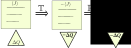
\includegraphics{../images/PT-Transform.pdf}
 % PT-Transform.pdf: 372x138 px, 72dpi, 13.12x4.87 cm, bb=0 0 372 138
 \caption[Illustration of symmetric and asymmetric observables under time reversal and space inversion. ]{Illustration of observable mechanical flux in the system $\langle J \rangle$ and heat exchange with a reservoir $\Delta Q$ under 
     time reversal $(\mathbb{T})$ and space inversion $(\mathbb{P})$. The mechanical flux 
     is symmetric under $\mathbb{P}\mathbb{T}$-transformation, the heat exchange is anti-symmetric. }
 \label{fig:PTtransform}
\end{figure}

Jack and Evans showed that constraints symmetric under time reversal $(\mathbb{T})$ and space inversion $(\mathbb{P})$  induce undesired symmetries in the system~\cite{jack2016absence}.  These symmetries imply that heat exchange with the reservoir averages to 0 in the implied ensemble. It follows that the system is in equilibrium with its reservoir and symmetric constraints cannot form NESS-ensembles. Figure \ref{fig:PTtransform} illustrates how the mechanical flow $\langle J \rangle$ and heat exchange with a reservoir $\Delta Q$ transform  respectively: Both, the mechanical flow and the heat transfer picks up a minus under time reversal, but only the mechanical flow is negative under space inversion too. The heat flow is unaffected by space inversion; the  heat $\Delta Q$ is an asymmetric and the mechanical flow $\langle J \rangle$ is a symmetric constraint. The symmetry of the flux under $\mathbb{PT}$-transform passes onto the resulting distribution of trajectories when enforced in the Maximum Caliber
\begin{equation}
    \mathcal{C_{\text{J}}} = \int \diff \Gamma \; p[\Gamma] \ln \left ( \frac{ p[\Gamma]}{q[\Gamma]} \right )  
- \zeta \left ( \int \diff \Gamma \; p[\Gamma] - 1 \right ) \\
- \nu \left( \int \diff \Gamma \; p[\Gamma] J[\Gamma] - \langle J \rangle \right),
\end{equation}
resulting in the distribution
\begin{equation}
    p[\Gamma] = \frac{q[\Gamma]}{Z(\nu)} \exp \left ( -\nu J[\Gamma]  \right ) ,
    \label{eq:LDT}
\end{equation}
where $Z(\nu) = \int \diff \Gamma q[\Gamma] \exp \left ( -\nu J[\Gamma]  \right ) $,
so one can conclude 
\begin{equation}
    \begin{aligned}
  p[ \mathbb{PT} \Gamma] &= \frac{q[\mathbb{PT} \Gamma]}{Z(\nu)} \exp \left ( -\nu J[\mathbb{PT} \Gamma]  \right )\\
  &= \frac{  q[\mathbb{PT} \Gamma]}{Z(\nu)} \exp \left ( -\nu J[ \Gamma]  \right )
\end{aligned}
\end{equation}
The symmetry is exploited when 
calculating the average heat exchanged with the reservoir in the target ensemble by
\begin{equation}
 \begin{aligned}
  \langle \Delta Q \rangle &= \int \diff \Gamma p[\Gamma] \Delta Q[\Gamma] \\
  &= \frac{1}{2}\int \diff \Gamma \frac{\Delta Q[\Gamma]}{Z(\nu)} 
  \exp \left ( -\nu J[\Gamma] \right ) \left ( q[\Gamma] - q[\mathbb{PT} \Gamma] \right ) \\
  &= 0 \;\;\;\;\;\;\;\; \text{if} \;\;\;\; q[\Gamma] = q[\mathbb{PT} \Gamma].
\end{aligned}
\end{equation}
Note that $q[\mathbb{PT} \Gamma]= q[\Gamma]$ is only valid if the reference data fulfils detailed balance, i.e. in equilibrium. The last statement shows that no heat in the final system can be dissipated in case the reference data is equilibrated, 
i.e. we cannot draw off-equilibrium information from equilibrium data. A trajectory ensemble created with evenly distributed $q[\Gamma]$ does not interchange heat either. Jack and Evans conclude that the chosen constraint is insufficient to describe off-equilibrium states~\cite{jack2016absence}. A Caliber with only symmetric constraints can be discarded for off-equilibrium. However,  the Caliber combined with asymmetric constraints and possibly symmetric constraints can dissipate heat~\cite{agozzino2019minimal}.

Lastly, we will distinguish between local and global constraints. Quantities may be constrained on the whole system, like energy or mechanical flow in the previous example. There are attempts to constrain the system on a smaller level, e.g. in detailed balance~\cite{wan2016maximum,rudzinski2016communication}. There is no a priori statement one can make about global or local constraints. Global constraint are easier to infer because they are less prone to fluctuation and use one constraint per quantity, whereas local constraints use many constraints. On the other hand, path dependence of off-equilibrium processes suggests that local constraints are more promising. For a dissipating system, it does matter where and when heat is transferred to or from the reservoir. Whereas the time point does not matter for NESS, the position does. The following section shows examples of local and global constraints on the Maximum Caliber.  

\subsection{Application of Constraints}
The previous discussion gives an idea of how to choose constraints: In the best case, one chooses an extensive quantity to avoid errors due to missing higher-order constraints. At least one asymmetric constraint is needed to break $\mathbb{PT}$-symmetry. A candidate that fulfils both conditions is the entropy production or, similarly, the heat dissipated in the full system. Similar to the picture of a canonical ensemble, we think of the system being connected to a reservoir. The reservoir for a NESS has two tasks: One is to provide the system with heat to maintain its state away from equilibrium. The other is to withdraw the same amount of heat from the system, the system itself does not dissipate any heat. This type of reservoir is modelled by constraining the amount of heat flow to or from the system. Fluctuations are allowed because the average of the heat flows is constraint. An open question is whether a global heat reservoir is modelled for the whole system or if the heat reservoir acts local depending on the state of the system.  

The assumption of constraining global and local energy productions is tested on the minimal model introduced in section \ref{sec:1Dmodel}. Furthermore, the system is constrained to the global balance condition in the last case. The constraints are tested by simulating two systems, one in equilibrium and one under external driving. The dynamics and statics are reweighted into each other. Static information are presented by the stationary distribution profile, dynamic information by the first passage-time distribution (FPTD) between the metastable states of the system. If static and dynamic information are recovered, the chosen constraints are considered sufficient for the simplified system. 

\subsubsection{Global Entropy Production}
Global entropy production for a Markovian system can be described by 
$\langle \Delta S \rangle = \sum_{i,j}  \pi_i p_{ij} \ln  \Delta S_{ij} $, where $\Delta S_{ij}$ 
is the local entropy production when going from state $i$ to state $j$. This quantity is discussed in section \ref{sec:1Dmodel} along with the model, where the start and endpoint are the middle of the microstates respectively. The global entropy production $\langle \Delta S \rangle$ is given by the target state that we want to reweight to. 
Enforcing the single global reservoir on the Caliber gives 
\begin{equation}
\begin{aligned}
 \mathcal{C}_{\Delta S} &= -\sum_{i,j} \pi_i p_{ij} \ln \frac{p_{ij}}{q_{ij}} 
      +  \sum_i \pi_i \mu_i \left( \sum_j p_{ij} - 1 \right) + \zeta \sum_i ( \pi_i -1) \\
      &+ \alpha \left ( \sum_{i,j}  \pi_i p_{ij} \ln \Delta S_{ij} - \langle \Delta S \rangle \right ).
\end{aligned}
\end{equation}
Note that the Lagrangian multiplier $\mu_i$ was rescaled by a factor $\pi_i$ without loss 
of generality.
With the requested maximisation $\pdv{ \mathcal{C}_{\Delta S}}{\pi_i}=0$ and 
$\pdv{ \mathcal{C}_{\Delta S}}{p_{ij}}=0 \;\; \forall i,j$ one finds
\begin{equation}
\begin{aligned}
0 &= - \sum_{k} p_{ik} \ln \frac{p_{ik}}{q_{ik}} + \zeta  
+ \alpha \sum_k p_{ik} \Delta S_{ik} \;\;\;& \forall i&\\
0 &= - \pi_i \ln \frac{p_{ij}}{q_{ij}}- \pi_i + \pi_i \mu_i  + \alpha \pi_i \Delta S_{ij} \;\;\;& \forall i,j& . 
\end{aligned}
\end{equation}
The second equation can be solved for 
\begin{equation}
 p_{ij} = q_{ij} \exp \left (-1+ \mu_i + \alpha \Delta S_{ij} \right ),
\end{equation}
which is plugged into the first equation resulting in
\begin{equation}
 \mu_i -1 = \zeta,
 \end{equation}
giving the final equation 
\begin{equation}
 p_{ij} = q_{ij} \exp \left (-1+ \zeta + \alpha \Delta S_{ij} \right ).
\end{equation}
The constraint on the global entropy production is not explicitly enforced and the Lagrangian multiplier $\alpha$ remains unsolved. $\zeta$ is a normalisation constant enforcing $\sum_i \pi_i = 1$. The Lagrangian multiplier $\alpha$ takes a similar role as the $\beta$ in the canonical ensemble. The $\beta$ is identified with the inverse temperature by comparison to thermodynamics and allows us physical intuition on its role. An easy interpretation of $\alpha$ is not given here and the value in the reference simulation is unknown. It is determined by numerical variation of $\alpha$ to cancel the deviation between the reweighted total entropy production and the total entropy production of the target system, as determined by the reference simulation. This will satisfy the last constraint of $\langle \Delta S \rangle$ on the Caliber.  
Figure \ref{fig:rewtrial1} shows that the reweighting fails for both the static and dynamic properties. 
We will turn to enforce the entropy productions on a local level.
\begin{figure}[t]
 \centering
 \includegraphics{../plots/Jaynes/fpt_J_2010_2910.pdf}
 % fpt_J_2010_2910.pdf: 0x0 px, 300dpi, 0.00x0.00 cm, bb=
 \caption[Stationary distribution and first-passage time distribution for the driven 1D system reweighted with respect to global entropy production.]{Comparing (a) the stationary distribution $p_s$ and (b) the FPTD $p_{\; \text{FPT}}$ for the process $B \rightarrow C$ of the equilibrium system ($f=0~\epsilon / \mathcal{L}$) and driven system ($f=9~\epsilon / \mathcal{L}$). The reweighting procedure tests the global entropy production of the target system as a defining system constraint.}
 \label{fig:rewtrial1}
\end{figure}
\subsubsection{Local Entropy Production}
Enforcing the local entropy production requires a Lagrangian multiplier at each transition. Determining a value for each transition means to couple the same reservoir at a different strength. 
The Caliber is defined by
 \begin{equation}
\begin{aligned}
 \mathcal{C}_{\Delta S_{ij}} &= -\sum_{i,j} \pi_i p_{ij} \ln \frac{p_{ij}}{q_{ij}} 
      +  \sum_i \mu_i \pi_i \left( \sum_j p_{ij} - 1 \right) + \zeta \sum_i ( \pi_i -1) \\
    &+ \sum_{i,j} \pi_i \alpha_{ij} \left ( \ln \frac{p_{ij}}{p_{ji}} -  \Delta S_{ij}  \right ),
\end{aligned}
\end{equation}
using the local entropy production relating the forward and backward 
jumping probability (see section~\ref{sec:NESS}). The Lagrangian multiplier $\alpha_{ij}$ and $\mu_i$ were rescaled by $\pi_i$.   
The maximisation with respect to the transition probabilities gives
  \begin{equation}
    0 = - \pi_i \ln \left ( \frac{p_{ij}}{q_{ji}} \right ) - \pi_i + \pi_i     \mu_i + \pi_i \frac{ \alpha_{ij} }{p_{ij}} - \pi_j \frac{ \alpha_{ji} }{p_{ij}}.
  \end{equation}
Solving for $p_{ij}$ with $\pi_i \neq 0$ 
  \begin{equation}
  p_{ij} = q_{ij} \; \exp \left ( -1 + \mu_i  + \frac{\gamma_{ij}}{p_{ij}} \right ),
\label{eq:pijearly}
  \end{equation}
where $\gamma_{ij} = \alpha_{ij} - \frac{\pi_j}{\pi_i} \alpha_{ji}$ is used.
Enforcing the local entropy productions explicitly by $\Delta S_{ij} = \ln \frac{p_{ij}}{p_{ji}}$ and after some algebra one finds
\begin{equation}
 \frac{\gamma_{ij}}{p_{ij}} = w_{ij} \left ( \Delta S_{ij} - \Delta S_{ij}^q -\mu_i + \mu_j \right ),
\end{equation}
where the definitions $w_{ij} = 1/\left(1 + \frac{\pi_i p_{ij}}{\pi_j p_{ji}} ) \right)$ and 
$\Delta S_{ij}^q = \ln \frac{q_{ij}}{q_{ji}} $ have been used. This expression is plugged into equation \ref{eq:pijearly} and using $w_{ij} + w_{ji} =1$ we  find
\begin{equation}
 p_{ij} = q_{ij} \exp \left ( -1 + w_{ji} \mu_i + w_{ij} \mu_j + w_{ij} (\Delta S_{ij} -\Delta S_{ij}^q)  \right ) 
\label{eq:pij2early}
\end{equation}
The Caliber maximisation with respect to the stationary distribution gives
  \begin{equation}
    \begin{aligned}
      0 =& -\sum_k p_{ik} \ln \left ( \frac{p_{ik}}{q_{ik}}  \right ) + \mu_i \sum_k p_{ik} - \mu_i  +\zeta  \\
      &+ \sum_{k} \alpha_{ik} \left( \ln \left ( \frac{p_{ik}}{p_{ki}} 
\right) - \Delta S_{ik}  \right  ) .
    \end{aligned}
  \end{equation}
  By plugging in equation \ref{eq:pijearly} and making use of the constraints, one finds a relation between the $\gamma_{ij}$ and $\mu_i$:
  \begin{equation}
    \mu_i  = 1 + \zeta + \sum_k \gamma_{ik}.
  \end{equation}
Defining $c_i = \sum_k \gamma_{ik} $ and plugging $\mu_i$ into equation \ref{eq:pij2early}
 results in the final equation
 \begin{equation}
 p_{ij} = q_{ij} \exp \left ( \zeta + w_{ji} c_i + w_{ij} c_j + w_{ij} (\Delta S_{ij} -\Delta S_{ij}^q)  \right ).
 \label{eq:altpij}
 \end{equation}  
The constraint of conserved transition probabilities $\sum_k p_{ik} =1 $ gives
 \begin{equation}
 1 = \sum_k q_{ik} \exp \left ( \zeta + w_{ki} c_i + w_{ik} c_k + w_{ik} (\Delta S_{ik} -\Delta S_{ik}^q)  \right ).
 \end{equation}
 This equation can be solved for $\bm{c}$ by  numerical iteration, discussed in the following section \ref{sec:numerics}.
 The result of enforcing local entropy productions is shown in figure \ref{fig:rewtrial2}. The stationary distribution is reproduced correctly by the reweighting procedure, showing a significant improvement compared to the global constraint. The dynamics are not reproduced correctly, indicating that the current model of a reservoir providing heat locally is not sufficient. 
 
  \begin{figure}[t]
 \centering
 \includegraphics{../plots/Jaynes/fpt_Sloc_2010_2910.pdf}
 % fpt_J_2010_2910.pdf: 0x0 px, 300dpi, 0.00x0.00 cm, bb=
 \caption[Stationary distribution and first-passage time distribution for the driven 1D system reweighted with respect to local entropy production.]{Comparing (a) the stationary distribution $p_s$ and (b) the FPTD $p_{\; \text{FPT}}$ for the process $B \rightarrow C$ of the equilibrium system ($f=0~\epsilon / \mathcal{L}$) and driven system ($f=9~\epsilon / \mathcal{L}$). The reweighting procedure tests local entropy productions of the target system as a defining system constraint.}
 \label{fig:rewtrial2}
\end{figure}
\subsubsection{Local Entropy Production and Global Balance}
The previous constraints define the interaction on every transition with the reservoir but the influence of local changes on the whole system are not modelled. We add global balance $\pi_i = \sum_k \pi_k p_{ki} \; \forall i$ as a condition for NESS (see section~\ref{sec:NESS}) to the list of constraints. It connects a single state on the left-hand side of the equation to all other states of the global system on the right-hand side. Furthermore, it builds a connection between stationary and dynamic probabilities that were previously maximised without specific coupling. The full Caliber is given by
  \begin{equation}
    \begin{aligned}
      \mathcal{C} = -&\sum_{i,j} \pi_i p_{ij}\ln \frac{p_{ij}}{q_{ij}} 
      +   \sum_i \mu_i \pi_i \left( \sum_j p_{ij} - 1 \right) + \zeta ( \sum_i \pi_i -1) \\
      +&  \sum_j \pi_j \nu_j \left(\sum_i \pi_i p_{ij} - \pi_j \right) 
      + \sum_{ij} \pi_i  \alpha_{ij} \left( \ln \left( 
\frac{p_{ij}}{p_{ji}} \right) - \Delta S_{ij} \right).
    \end{aligned}
  \end{equation}
The maximisation is performed equivalently to the derivation without global balance, just with additional Lagrangian multiplier $\nu_i$. The maximisation with respect to transition probabilities equivalent to equation \ref{eq:pijearly} becomes
  \begin{equation}
  p_{ij} = q_{ij} \; \exp \left ( -1 + \mu_i + \nu_j + \frac{ \gamma_{ij} 
}{p_{ij}} \right ).
  \label{eq:pij}
  \end{equation}
The maximisation of the Caliber with respect to the stationary distribution 
shows
  \begin{equation}
    \begin{aligned}
      0 =& -\sum_k p_{ik} \ln \left ( \frac{p_{ik}}{q_{ik}}  \right ) + \mu_i 
\sum_k p_{ik} - \mu_i \\& +\zeta + \sum_k \nu_k p_{ik} - \nu_i 
      + \sum_{k} \alpha_{ik} \left( \ln \left ( \frac{p_{ik}}{p_{ki}} 
\right) - \Delta S_{ik}  \right  ) .
      %\\ & + \gamma \sum_k p_{ik} F_{ik} 
    \end{aligned}
  \end{equation}
  By making use of the constraint $\sum_k p_{ik}=1$ and equation \ref{eq:pij} one finds a relation between the Lagrangian multipliers $\gamma_{ij} = \alpha_{ij} - \frac{\pi_j}{\pi_i} \alpha_{ji}$, $\mu_i$ and $\nu_i$:
  \begin{equation}
    \mu_i + \nu_i = 1 + \zeta + \sum_k  \gamma_{ik}
  \label{eq:minpi}
  \end{equation}
  Making use of equation \ref{eq:pij} to enforce the local entropy productions $\Delta S_{ij} = \ln \frac{p_{ij}}{p_{ji}}$, where $\Delta S_{ij}^q = \ln \frac{ q_{ij}}{q_{ji}}$ denotes the reference entropy production and the definition $w_{ij} = 1/\left(1 + \frac{\pi_i p_{ij}}{\pi_j p_{ji}} ) \right)$ is used again
    \begin{equation}
    \frac{ \gamma_{ij}}{p_{ij}} = w_{ij} \left ( \Delta S_{ij} - \Delta 
S_{ij}^q -\mu_i +\mu_j -\nu_j +\nu_i \right ).
      \label{eq:alpha}
    \end{equation}
Plugging this result into equation \ref{eq:pij} gives
\begin{equation}
  p_{ij} = q_{ij} \; \exp \left ( -1 + w_{ji} \mu_i + w_{ij} \mu_j 
  + w_{ji} \nu_j + w_{ij} \nu_i + w_{ij} ( \Delta S_{ij} - \Delta S_{ij}^q )  \right ) . 
\label{eq:pij2}
\end{equation}
Enforcing the constraint $\sum_k p_{ik} =1 $ results in a set of 
N equations, where $N$ is the number of microstates. Combined with equations~\ref{eq:minpi} there is a set of $2N$ non-linear equation to be solved.
 \begin{figure}[t]
 \centering
 \includegraphics{../plots/Jaynes/ratio_all.pdf}
 % fpt_J_2010_2910.pdf: 0x0 px, 300dpi, 0.00x0.00 cm, bb=
 \caption[Transition probability matrix of the 1D driven system and the violation of detailed balance.]{(a) the transition probabilities for the driven system ($f=9~\epsilon / \mathcal{L}$). (b) the deviation from detailed balance in the form $\log_{10} \frac{\pi_i p_{ij}}{\pi_j p_{ji}}$. The black regions around $0$ indicate that detailed balance holds approximately, red regions indicate violation of detailed balance. The matrix is antisymmetric by definition.}
 \label{fig:Sprod}
\end{figure}
In order to do that, we approximate that the deviation from detailed balance is small. Mathematically we assume that $\frac{\pi_i p_{ij}}{\pi_j p_{ji}} \approx 1 $, resulting in $w_{ij} \approx \frac{1}{2}$.  The approximation close to detailed balance is applied for a single Markovian jump --- a trajectory consists of many jumps and can grow large entropy productions despite the approximation. 
Figure~\ref{fig:Sprod} illustrates that this is a reasonable approximation for the important transitions where $p_{ij}$ is large.  
\begin{figure}[t]
 \centering
 \includegraphics{../plots/Jaynes/fpt_2010_2910.pdf}
 % fpt_J_2010_2910.pdf: 0x0 px, 300dpi, 0.00x0.00 cm, bb=
 \caption[Stationary distribution and first-passage time distribution for the driven 1D system reweighted with respect to local entropy production and global balance.]{Comparing (a) the stationary distribution $p_s$ and (b) the FPTD $p_{\; \text{FPT}}$ for the process $B \rightarrow C$ of the equilibrium system ($f=0~\epsilon / \mathcal{L}$) and driven system ($f=9~\epsilon / \mathcal{L}$). The reweighting procedure with local entropy production of the target system and global balance  recovers dynamics and statics well.}
 \label{fig:rewtrial3}
\end{figure}
Using the approximation on equation \ref{eq:pij2} gives
    \begin{equation}
      p_{ij} = q_{ij} \exp \left ( \frac{1}{2} \left ( -2 + \mu_i +\nu_j +\mu_j 
+ \nu_i + \Delta S_{ij} - \Delta S_{ij}^q \right ) \right ).
    \end{equation}
    Using the result of equation \ref{eq:minpi} and the definition $c_i = \sum_k \gamma_{ik}$ shows
    \begin{equation}
    \begin{aligned}
    p_{ij} =& q_{ij} \exp \left ( \zeta+ \frac{1}{2} \left ( c_i + c_j + \Delta
S_{ij} - \Delta S_{ij}^q \right ) \right ) \\
=&     \sqrt{q_{ij} q_{ji} } \exp \left ( \zeta+ \frac{1}{2} \left ( c_i + c_j + \Delta
S_{ij} \right ) \right ). 
    \end{aligned}
    \label{eq:finalpij}
    \end{equation}
This shows that we have two options for the input parameters: The reweighting depends either on the total entropy production of the target system or the difference in local entropy production of target and reference system. 
The unknowns $\bm{c}$ are calculated by enforcing the relation 
$\sum_j p_{ij} =1 $
    \begin{equation}
      1 = \sum_j q_{ij} \exp \left ( \zeta+ \frac{1}{2} \left ( c_i + c_j + \Delta 
S_{ij} - \Delta S_{ij}^q \right ) \right ),
      \label{eq:iteration}
    \end{equation}
being a non-linear system of equations that can be solved numerically. It will be shown in section \ref{sec:numerics} that this set of equations in convex and has a unique solution, independent of initial conditions on the solving algorithm. $\zeta$ is a Lagrangian multiplier that can be set to $0$ because the corresponding constraint $\sum_k \pi_k = 1$ is implicitly met by the rowwise normalisation of the transition matrix and 
its enforced relation to the stationary distribution by global balance 
$\pi_i = \sum_k \pi_k p_{ki}$.  The results of the reweighting procedure,using the approximated solution is given in figure \ref{fig:rewtrial3}. Both quantities are estimated correctly reweighted from equilibrium to off-equilibrium and vice versa, indicating that the combination of local entropy production and global balance as constraint apply for this system. 

The outcome of the Caliber maximisation without global balance in equation \ref{eq:altpij} is equivalent to the final equation \ref{eq:finalpij} when the same approximation $w_{ij} \approx \frac{1}{2}$ is applied. It  can thus not be argued that the global balance condition is indeed essential for the reweighting process, but we can argue that local entropy productions alone are not sufficient. It is possible that another constraint, which could not be identified, leads to equation \ref{eq:finalpij} without approximation. A possible candidate is a reservoir not connected to the transition, but to the single states of the system. An indicator are the responsible $N^2$ Lagrangian multipliers $\alpha_{ij}$ not being calculated in the maximisation because they are reduced to the $N$ parameters $c_i$. It follows that only the strength of coupling to each state is calculated separately.

We will stick to to the given equation for this thesis because it produces excellent, fast and unique results for different systems. The presented set of non-linear equations without approximation may not have a unique solution and is too complex for fast application. The  enforced constraints on the entropy production hold true with a relative error less than $ 10^{-9}$, 
indicating the approximation applies for the given system. This test can be run for every system the algorithm is applied to.  However, a full solution in agreement with the approximated form would prove that global balance is essential for reweighting. It would also give mathematical ground to apply the reweighting procedure to systems under stronger driving.  


\subsection{Invariant Measure}
\label{sec:Invariant}
Reweighting suggests that there is an underlying quantity that is the same for all systems. For Equilibrium systems, it is the density of states. Once it is known one can construct the system at any thermodynamic point, because the quantity is independent of the ensemble and the microstate weigthing of the ensembles is known. For the current reweighting scheme, we expect an underlying invariant too. It does not have to be completely independent of thermodynamics, only of the quantities that are altered by reweighting. The temperature for instance is constant for all systems.

Starting with the reweighting formulae in equation~\ref{eq:finalpij}, the product of forward and backward transition is denoted by
  \begin{equation}
    p_{ij} p_{ji} = q_{ij} q_{ji} \exp ( c_i + c_j + 2 \zeta ),
    \label{eq:pp}
  \end{equation}
where the symmetry of local entropy production is used to cancel $\Delta S_{ij} =- \Delta S_{ji}$. Similarly, we may reweight the other way round from $q_{ij}$ to $p_{ij}$ with another set of constants $\mathbf{\tilde c}$:
  \begin{equation}
    q_{ij} q_{ji} = p_{ij} p_{ji} \exp ( \tilde c_i + \tilde c_j + 2 \tilde 
\zeta  ) .
    \label{eq:qq}
  \end{equation}
  Combing both equation~\ref{eq:pp} and \ref{eq:qq} results in:
  \begin{equation}
    - \tilde c_i - \tilde c_j - 2 \tilde \zeta = c_i + c_j + 2 \zeta.
  \end{equation}
Using this result to plug into equation~\ref{eq:pp}, the expression 
  \begin{equation}
    I_{ij}^2 = p_{ij} p_{ji} \exp \left ( \frac{\tilde c_i + \tilde c_j}{2} +\tilde 
\zeta \right ) 
= q_{ij} q_{ji} \exp\left ( \frac{ c_i + c_j}{2}+ \zeta \right )
  \end{equation}
is invariant under reweighting. It is constant under different driving of the  system. Note that $I_{ij}$ is defined up to a constant $\zeta$. This quantity and its physical meaning will be discussed in detail in section~\ref{sec:InvariantC}. 
 
\subsection{Numerical Maximisation}
\label{sec:numerics}
For an exact solution of the set of $2N$ equations 
\begin{equation}
 \begin{aligned}
 0 &=\sum_k^N q_{ik} \; \exp \left ( -1 + w_{ik} \mu_k + w_{ki} \mu_i 
  + w_{ik} \nu_i + w_{ki} \nu_k + w_{ik} ( \Delta S_{ik} - \Delta S_{ik}^q )  \right )  \\
0&= - \mu_i - \nu_i + 1 + \zeta + \sum_k^N p_{ik} w_{ik} \left ( \Delta S_{ik} - \Delta S_{ik}^q -\mu_i +\mu_k -\nu_k +\nu_i \right )    
 \end{aligned}
\label{eq:fullsol}
\end{equation}
has to be solved for the Lagrangian multiplier vectors $\bm{\mu}$ and $\bm{\nu}$. The Kullback-Leibler divergence alone is a convex function, but constraining to the non-linear local entropy production introduced non-convexity. It is not a priori known if there is a unique solution of the equations. Finding an analytic solution failed, so we solve it by numerical methods. 

The analytic solution expanded $w_{ij} = 1/\left(1 + \frac{\pi_i p_{ij}}{\pi_j p_{ji}} ) \right)$ around detailed balance. It will be shown in the following that the resulting set of equations becomes convex and possible solutions for higher order expansion will be suggested.  


\subsubsection{0th Order Expansion}
The system of equations \ref{eq:iteration} resulting from the 0th order expansion are rewritten by the definitions $\Phi_i = \exp (c_i/2 )$ and $A_{ij} = q_{ij}\exp \left ( \zeta+ \frac{1}{2} \left (  \Delta S_{ij} - \Delta S_{ij}^q \right ) \right )$. 
The equations \ref{eq:iteration} become 
\begin{equation}
  \Phi_i = \frac{1}{\sum_k A_{ik} \Phi_k}.
\end{equation}
We define this function as $f_i= \Phi_i$ and show that it is convex by calculating the Hessian
\begin{equation}
    \frac{\partial^2 f}{ \partial \Phi_m \partial \Phi_n} =  \frac{2 A_{im} 
A_{in}}{\left ( \sum_k A_{ik} \Phi_k \right )^3}.
\end{equation}
Noting that $\Phi_i  \geq 0$ and $A_{ij} \geq 0$, the Hessian is 
positive definite and the function is convex. This means that a random starting point for $\Phi_i^{(0)}> 0$  can be chosen to find a numerical solution to this problem. We found that the least squared method with the implementation in pythons library \lstinline{scipy.optimize.least_squares}~\cite{branch1999subspace} and $\Phi_i\geq 0$ bounded below  gives the most robust result. 

\subsubsection{Full Solution}
We briefly show why the approximated solution is used throughout the thesis by attempting to solve the exact set of equation. The methods are applied to the testing system with 30 microstates by reweighting equilibrium data to itself.  We tried different numerical methods provided by scipy including:
\begin{itemize}
 \item Root finder (\lstinline{scipy.optimize.fsolve}~\cite{more1980user},
 \lstinline{scipy.optimize.least_squares}~\cite{branch1999subspace})
 \item Function minimiser (\lstinline{scipy.optimize.minimize(method="L-BFGS-B")}~\cite{zhu1997algorithm})
 \item Basinhopping (\lstinline{scipy.optimize.basinhopping}~\cite{wales1997global})
\end{itemize}
The root finding method uses the equations~\ref{eq:fullsol} directly and solves the set of equations self-consistently until a root is found, similar to the self-iteration. The other two methods need an error function $\mathcal{E} = \sum_i^N g_i f_i$ for numerical minimisation, where $f_i$ represents one equation in \ref{eq:fullsol} and $g_i$ weights each function. All methods need an initial point to start the algorithm.  As discussed earlier, the functions are non-convex and may have more than one minimum. The basinhopping algorithm attempts to solve this problem by using random displacements of parameters followed by error-function minimisation. The algorithm combines multiple minimisations but is not guaranteed to find the global minimum. The prospect is better because the method becomes less dependent on its initial value for long runtime. 

The parameters $w_{ij}$ depend on the stationary distribution $\bm{\pi}$ of the target system. We use the stationary algorithm of the 0th-order approximation to estimate $\bm{\pi}$ as it shows excellent agreement with the values known from simulation for the testing system. In a general application, one could add 
the linear dependence $\sum_k \pi_k p_{ik} = \pi_i$ to the list of equations but this is set aside for now. Applying the algorithm to the original set of equations we find that the variables tend to diverge. This problem is solved by the transformation
\begin{equation}
 \begin{aligned}
  u_i &= \mu_i - \nu_i \\
  v_i &= \mu_i + \nu_i
 \end{aligned}
\end{equation}
resulting in the new set of equations
\begin{equation}
\begin{aligned}
0 &= \sum_k q_{ik} \exp \left ( -1 + \frac{1}{2} \left( v_i + v_k +u_i -u_k \right ) + w_{ik} \left( -u_i + u_k + \Delta S_{ik} - \Delta S^q_{ik} \right) \right ) \\
0 &= 1 + \zeta -v_i + \sum_k p_{ik} w_{ik} \left ( \Delta S_{ik} - \Delta S^q_{ik}  -u_i +u_k \right ) .
\end{aligned}
\label{eq:fullsolTra}
\end{equation}
Comparing these equations to the approximated solution using $w_{ij}\approx \frac{1}{2}$ in equation~\ref{eq:iteration} shows that $\bm{v}$ takes the role of $\bm{c}$, and $\bm{u}$ are the new set of constants. This provides a starting point for the iteration at $\bm{v}= \bm{c}$,  $\bm{u}=0$ and $\zeta =0$.  Note that this choice does satisfy the first set of equations~\ref{eq:fullsolTra} for reweighting in equilibrium (i.e. $w_{ij} = \frac{1}{2}$) but not the second set of equations. 

The transformation solves the problem of diverging variables but reveals that the algorithms are unable to find a solution that fulfils all constraints. The root-finding methods fail to converge. The minimisation methods reveal that most constraints are fulfilled but there are large local errors as shown in figure~\ref{fig:fullsol}. The location of these errors can be changed by reassigning weighting factors $g_i$ of the error function $\mathcal{E}$. The basinhopping algorithm can find solutions with lower error but non with error vanishing for a complete solution. 

 \begin{figure}[t]
 \centering
 \includegraphics{../plots/Jaynes/fullsol.pdf}
 % fpt_J_2010_2910.pdf: 0x0 px, 300dpi, 0.00x0.00 cm, bb=
 \caption[Deviation of constraints when attempting to find a full solution to the Caliber maximisation by numerical minimisation.]{Deviation of constraints solving the full set of equations~\ref{eq:fullsolTra}. \enquote{Norm} refers to the first set of equation, \enquote{stationary} to the second.  }
 \label{fig:fullsol}
\end{figure}


Since finding a full solution is burdensome, we attempt to find solutions for higher order expansions. Expanding $w(x)$ where $x=\frac{\pi_i p_{ij}}{\pi_j p_{ji}} $ around 1 for the higher orders gives
\begin{equation}
 w(x) \approx \frac{1}{2} - \frac{x}{4} +\frac{x^3}{48} + \text{h.o.}.
\end{equation}
The same initial values as for the attempt of full solution $\bm{v}= \bm{c}$, $\bm{u}=0$ and $\zeta =0$ are chosen. The idea is based on solving the system approximately for the 1st-order approximation, use the output for an initial guess on the 3rd order approximation and continue until a full solution is found. In practice this attempt suffers from local errors like the full solution. 

The above discussion indicates that a full solution is difficult to find or not existent. In either case, the solution given by the 0th order expansion shows excellent results and will be used throughout the paper. Finding a full solution is nevertheless desirable. If the full solution can be shown to be exact in the sense of reweighting data, it indicates that the global balance condition completes the set of constraint for a NESS.

%  
% \bibliography{/home/marius/PhD/Thesis/references.bib}
% \bibliographystyle{plain}
% \end{document}
% 
% 
% 
% 

















